% Summarize your report and reiterate key points.
In this project, we developed a machine learning algorithm that can classify product listings according to the type of product being sold.
Our algorithm consisted of a pipeline using TF-IDF for feature extraction, SVD for feature selection, and SVM for final classification.
We then used cross-validation to select hyperparameters and tune our algorithm.

% Which algorithms were the highest-performing? 
We also evaluated our algorithm in comparison to several other models:
\begin{itemize}
    \item{A baseline model that used simple string search}
    \item{SVM with a Chi-Squared test for feature selection}
    \item{Multinomial Naive Bayes}
\end{itemize}

Our algorithm had an accuracy of 77\% compared to the baseline accuracy of 62\%.
Our algorithm also outperformed the alternate SVM and multinomial models.

% Why do you think that some algorithms worked better than others?
Our algorithm was able to outperform the alternate models because it was able to take advantage of structure in the large unlabeled dataset.
In this project, we had a small amount of labeled data, and a very large amount of unlabeled data.
The SVD we use is performed on the unlabeled data, which helps to expose structure not captured by the labeled data.
We then project our labeled data onto the vector space chosen by the SVD and train our SVM on the result.
This allows to take advantage of both our unlabeled and labeled data in selecting our decision boundry.

\begin{figure}[htbp]
    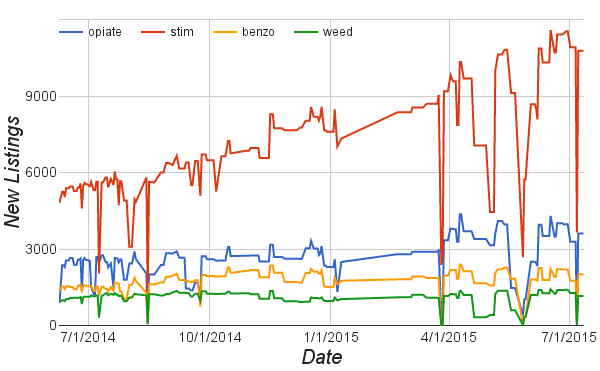
\includegraphics[width=\linewidth]{plots/new_categories_graph}
    \caption{New Listings By Category On Agora}
\end{figure}

We also used our classifier to measure the number of new products by category over time.
We found that by far the most common product listed on Agora is stimulants.
Interestingly, this was significantly different than an earlier anonymous market, The Silk Road,
where marijuana was the most common listed product, with stimulants a distant fourth\cite{christin-silkroad}.

This also matches reports from user and vendor forums, many of whom have complained that the
legalization of marijuana has reduced the profitability of selling online.
Conversely, amphetamine demand has dramatically risen, while production costs have dropped.
This has resulted in an apparent increase in product listings.
As far as we are aware, we are the first to rigorously document this switch.
This shows that our algorithm is extremely useful in practice, particularly for law enforcement and researchers.

